\chapter{PyBEL Tools}
\label{ch:pybel_tools}

The following section describes a subset of the functions and workflows that have been developed to assess, enrich, and analyze knowledge assemblies parsed by PyBEL. All code is made available as open source and stored in the PyBEL Tools repository (https://github.com/pybel/pybel-tools) on GitHub. Like PyBEL, it is thoroughly documented as to allow for the community to build upon it.

\section{Critical Assessment of Networks}
Before knowledge assemblies can be used to help interpret data, their validity and robustness must first be quantified. While many dimensions can be explored during this quantification, this section places focus on the identification of biological network motifs that indicate inconsistencies in the knowledge assembly. Network motifs have been studied in the context of transcriptional and phosphorylation networks \cite{Alon2007} and already provide insight to the biological activity. As knowledge networks add the heterogeneity of edges including correlative relationships, many new motifs must be identified and their effects inferred. This section presents the first portions of a taxonomy for network motifs in knowledge assemblies, interpret their effects, and use them assess the \ac{NeuroMMSig} knowledge base.

\subsection{A Taxonomy of Knowledge Assembly Motifs}

The first and most simple motif is a contradictory pair. These occur when there exist multiple edges between a given source and target that have conflicting relations, such as increases vs. decreases. However, contradictory pairs are not canonically invalid. They may arise from the effects of the biological context under which different relations were observed. These cases must be carefully considered.

There are many aspects that can be considered to resolve conflicts that cannot be explained by different biological scenarios. First, the date of publication can be considered. The most recent publication is most likely to have made use of other knowledge available to researchers, and be more right. Alternatively, if many publications were made with conflicting views in a short amount of time, the impact factor of the corresponding citations' journals can be considered.  

While there exists a single motif for identifying contradictory pairs, multiple motifs comprise the set of contradictory triplets. The algorithms that identify these triangles within a network come from a deep graph theoretic background to identify logically inconsistent relations. Because BEL knowledge graphs contain both causal and correlative relations, they can be analyzed jointly. The most simple is a mutually unstable triplet, which occurs when entities A, B, and C all negatively correlate with each other. Similarly, separately unstable triplets occur when A positively correlates with both B and C, but B and C are negatively correlated. Three more triple types are identified where a mix of  correlative and causal relations do not match: increase mismatch triplets, decrease mismatch triplets, and jens triplets.

Alternatively, stability analysis can be conducted to identify elements that are likely to be regulated by other parts of a system. These elements are particularly interesting because of the high impact that any given edge could have that connects to it. There are two types of unstable pairs: chaotic pairs, where A and B both increase each other and dampened pairs, where A and B both decrease each other. The same logic extends to chaotic triplets and dampened triplets. Interestingly, analyses of many knowledge assemblies seldom identified dampened triplets; possibly indicating their biological novelty. Chaotic and dampened cycles of length 4 and above are not identified, because the average number of possible connections at those lengths makes qualitative biological interpretation prohibitively difficult. 

Table 9 presents statistics over the occurrence of various network motifs in the three knowledge assemblies produced during the AETIONOMY project. While each case, such as mutually unstable triples, might be interesting, this provides direct insight into the large amount of effort necessary to investigate each unstable motif and motivates the further development of automated approaches for quantifying the robustness of a given knowledge assembly.

\begin{table}
\centering
\caption[Stability Analysis of NeuroMMSig]{Stability analysis statistics over the AETIONOMY knowledge assemblies for Alzheimer's disease, Parkinson's Disease, and Epilepsy. The ratios suggest that the relative counts of each network motif are not similarly correlated with network size or density. }
\label{tab:stability}
\def\arraystretch{1.5}
\begin{tabular}{p{55mm} p{25mm} p{25mm} p{25mm}}
 & \ac{AD} Knowledge Assembly v4.0.3 & Epilepsy Knowledge Assembly v1.1.2 & \ac{PD} Knowledge Assembly v1.1.1 \\
Chaotic Pairs & 56 & 12 & 16 \\
Chaotic Triples & 115 & 27 & 11 \\
Contradictory Pairs & 68 & 18 & 26 \\
Dampened Pairs & 7 & 2 & 4 \\
Dampened Triples & 1 & 0 & 2 \\
Decrease Mismatch Triples & 20 & 0 & 6 \\
Increase Mismatch Triples & 51 & 4 & 20 \\
Jens Unstable Triples & 657 & 153 & 85 \\
Mutually Unstable Triples & 2 & 0 & 7 \\
Regulatory Pairs & 19 & 9 & 15 \\
Separately Unstable Triples & 16 & 0 & 16
\end{tabular}
\end{table}

\subsection{Discussion}

As data integration projects like Bio2BEL make more data accessible during analysis, further plausibility and stability checks can be performed. One would be to integrate the data from \ac{UniProt} for each function and traverse the Gene Ontology molecular function annotations to identify properly annotated activities and flag improperly annotated ones to be either proposed as new, or fixed. Another example would be to check that protein and gene modifications are annotated properly using \ac{UniProt} and dbSNP, respectively. Adding additional checks using prior knowledge makes \ac{BEL} curation much more accessible to curators with less biological knowledge and also text mining systems that currently have less biological intuition.

\section{Survey of Algorithms}

Algorithms for analyzing pathways and networks can be categorized into three main categories: \ac{ORA}, \ac{FCS}, and \ac{PT} \cite{Khatri2012}. Over-representation analysis often focuses on the number of differentially expressed genes present or absent in a gene set compared to chance, while functional class scoring is less susceptible to large effects and considers the aggregate of groups of small effects. Pathway topology finally considers the biological relations between members of the pathway during analysis.

Furthermore, there is a distinction between methods that rely on the assumption that protein activities are correlated with their corresponding \ac{mRNA}s' expression changes (forward reasoning) versus the effect that upstream controllers of \ac{mRNA} expression have (backwards reasoning) \cite{Martin2014}

These algorithms have been developed for a wide variety of applications, data formats, and graph types. While many are heterogeneous, below are the most notable algorithms specific to networks from knowledge assemblies encoded in \ac{BEL}.

\subsection{Reverse Causal Reasoning}

Reverse causal reasoning (\ac{RCR}) is an approach to identify the upstream controllers of biological patterns measured in an experiment; often differential gene expression experiments between healthy and diseased patients. First, large knowledge assemblies are dissected into smaller hypothesis networks with one upstream node with multiple outgoing causal relations to target nodes represented by the experimental data set. Each hypothesis network is scored by its concordance between the observed up- and down-regulations of targets nodes to the sign of the causal relation and by its richness, or the explanatory power of the hypothesis network \cite{Catlett2013}. An example hypothesis network is shown in Figure 13.

\begin{figure}
\captionsetup{format=plain}
\makebox[\textwidth]{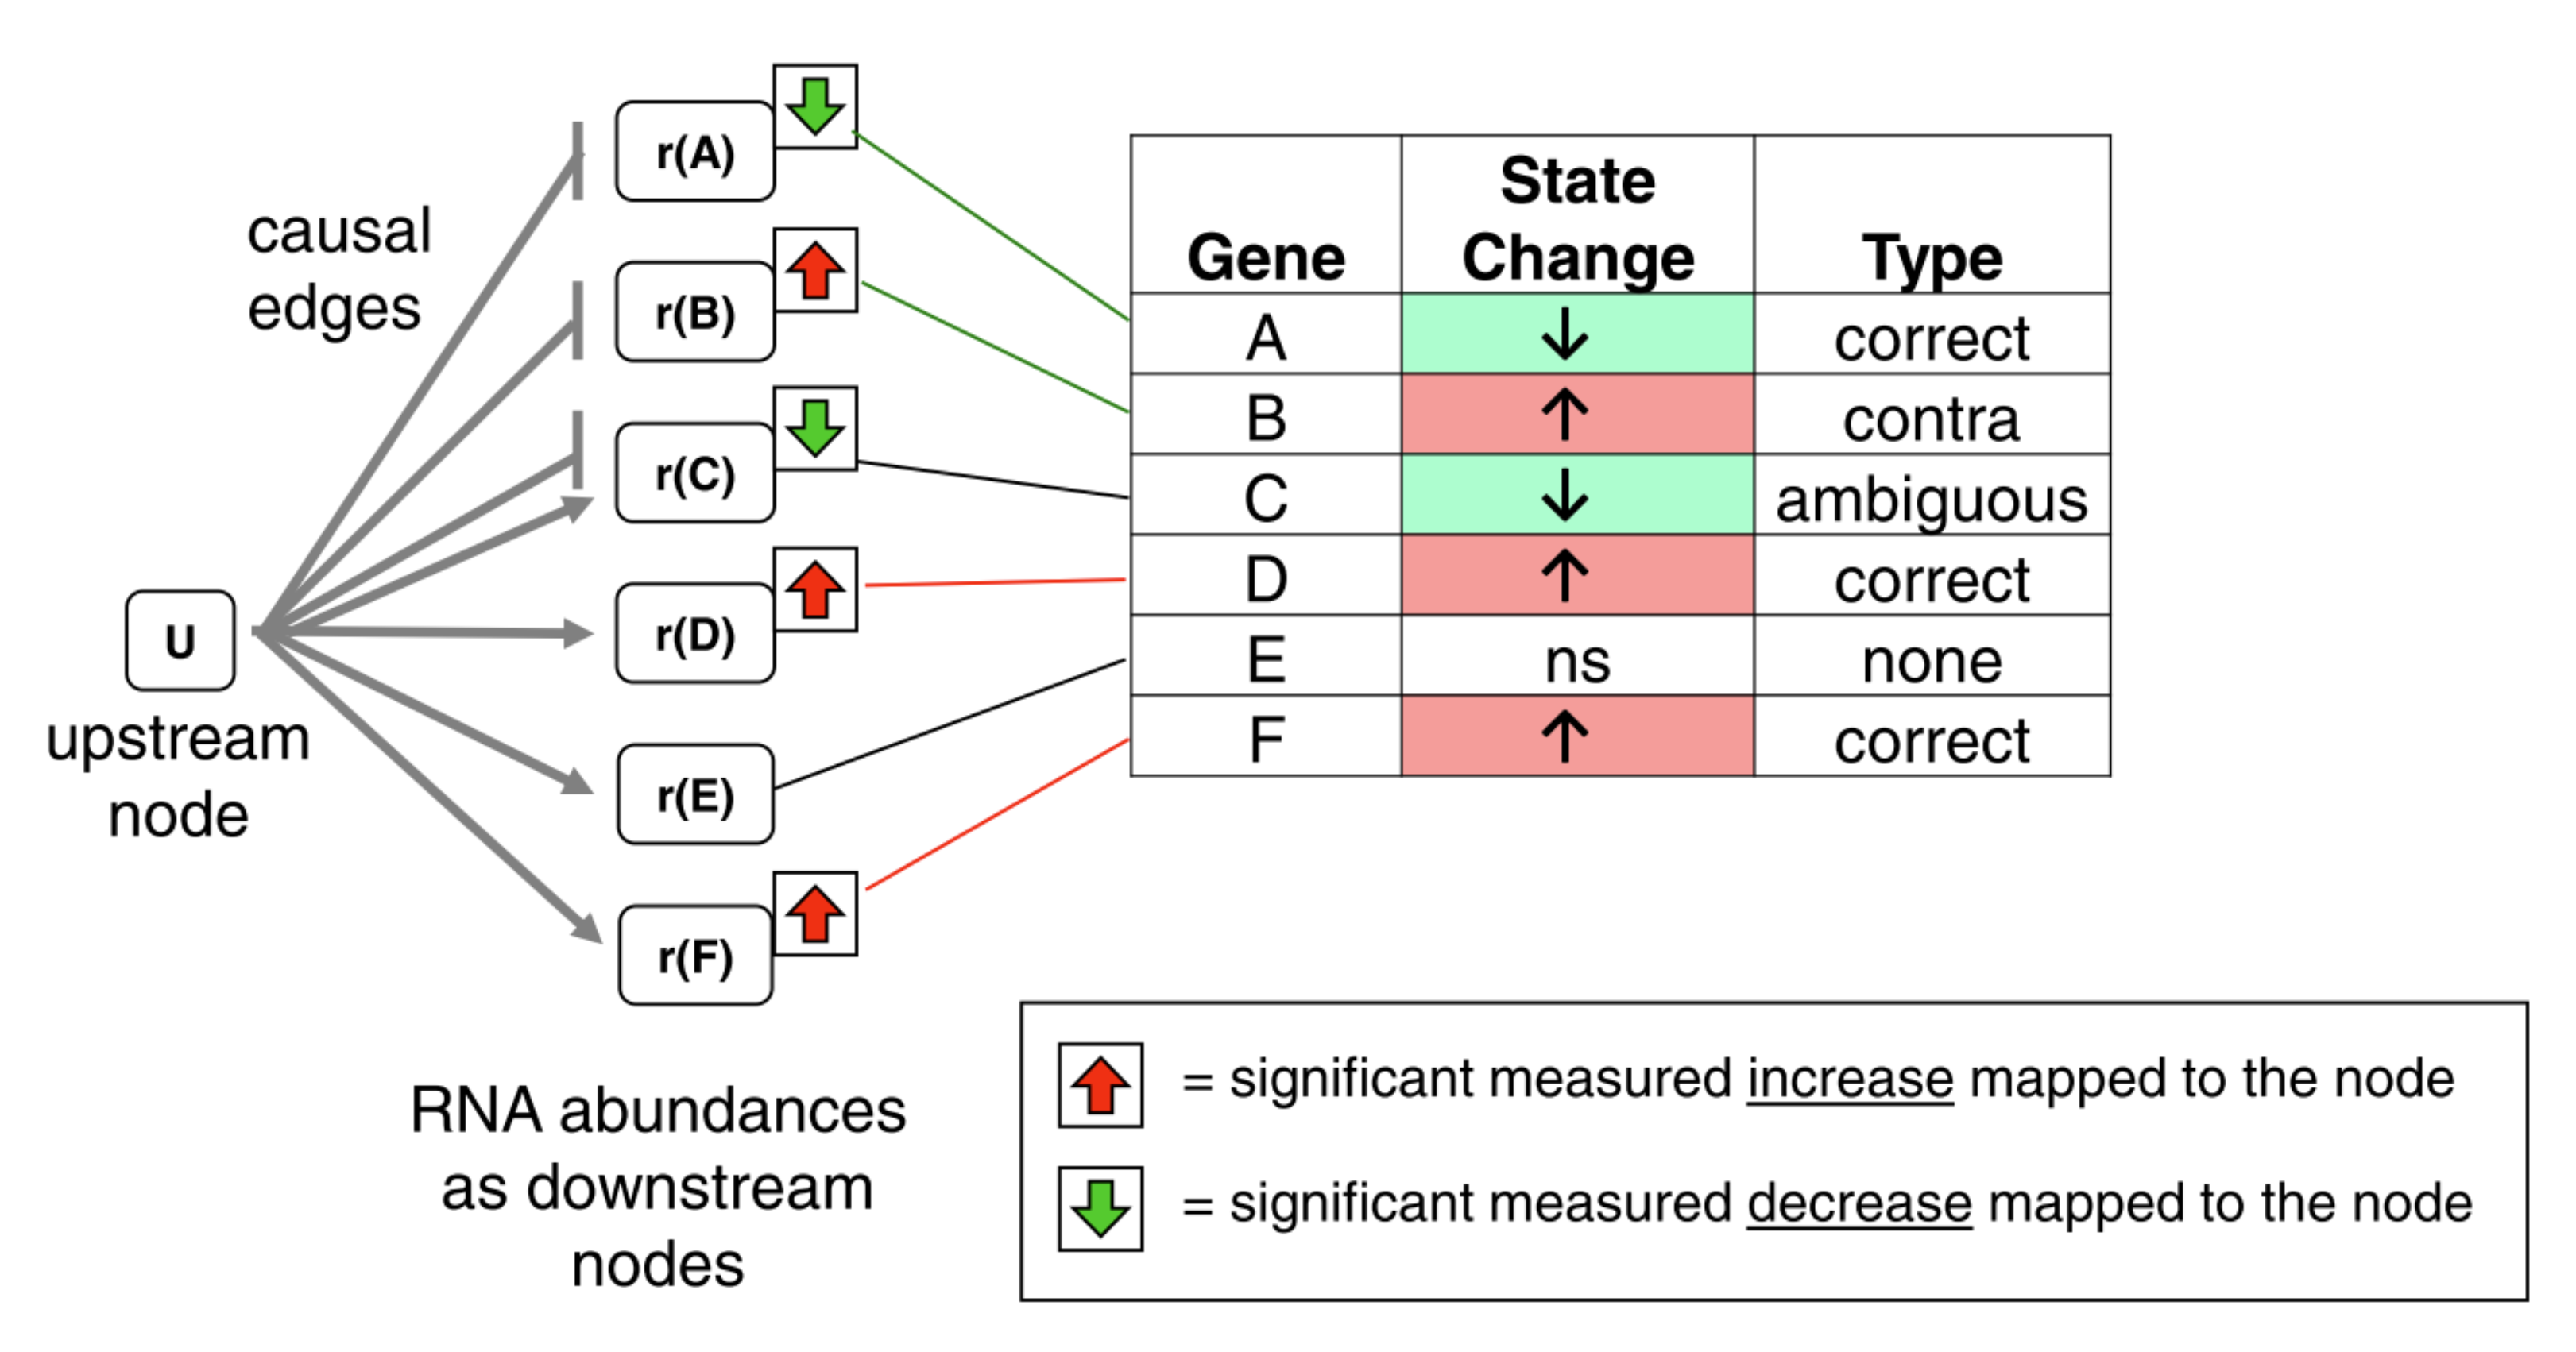
\includegraphics[width=160mm]{images/rcr_schematic.png}}
\caption[A Schematic Diagram of \ac{RCR}]{An example hypothesis network. Target nodes are counted as correct if they have a decreasing relationship and down-regulation, or an increasing relationship and up-regulation. Target nodes with multiple conflicting relationships are marked as ambiguous. Finally, target nodes are counted as incorrect if they have a mismatch between an increasing relationship and down-regulation, or a decreasing relationship and up-regulation. Adapted from \cite{Catlett2013}.}
\label{Fig:rcr_schematic}
\end{figure}

\subsection{Network Perturbation Amplitude}

While \ac{RCR} gives preliminary insights to significant biological controllers, it mostly ignores the topology of signaling, regulatory, and other causal networks that can be represented in knowledge assemblies (Figure 14). The \ac{NPA} measures the aggregated effect explained by the controller layer with reference to a given node with respect to their downstream nodes. Two complementary statistics for the effect of permutations of the upstream layer and downstream layer allow for further insight to the validity of \ac{NPA}s as a hypothesis generation mechanism \cite{Martin2014}.

\begin{figure}
\captionsetup{format=plain}
\makebox[\textwidth]{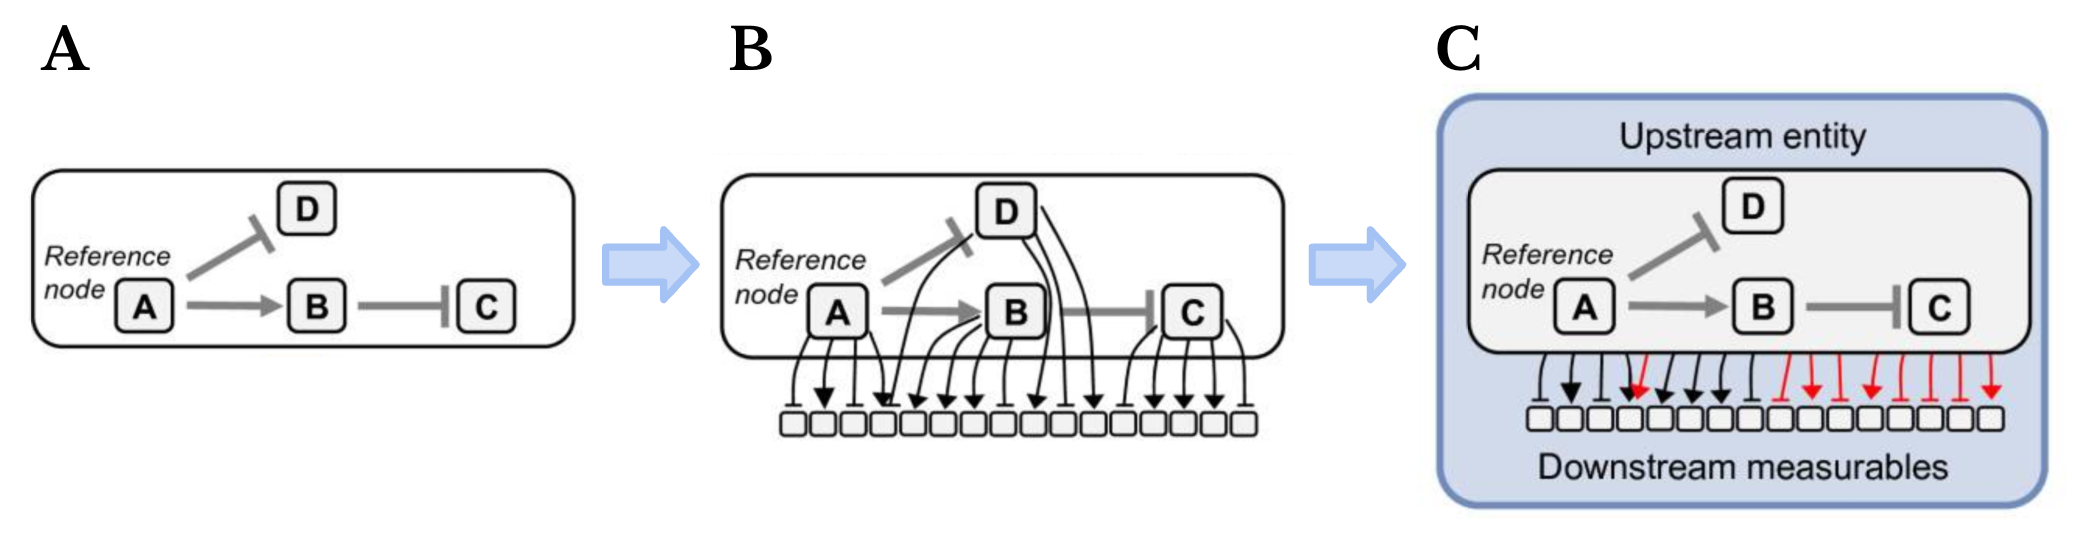
\includegraphics[width=160mm]{images/npa_schematic.png}}
\caption[Hypothesis Network Generation for Network Perturbation Amplitude]{Creation of hypothesis networks that accounts for the topology and interactions of  upstream controller layer with respect to a reference node A), their individual effects on the downstream layer B) and their combine effect C). Adapted from \cite{Martin2012}.}
\label{Fig:npa_schematic}
\end{figure}

\subsection{Sampling of Spanning Trees}

While \ac{NPA} enables more informed analyses than \ac{RCR}, its mathematical basis limits the topologies of knowledge networks that can be used to those with causal consistency. In these networks, all paths from one node to another result in the same aggregated effect of increases and decreases. An additional approach in Figure 15 for \ac{SST} with random walkers eliminates inconsistencies and can be aggregated over multiple trials to assign \ac{NPA} scores to networks that were otherwise inconsistent \cite{Vasilyev2014}. 

\begin{figure}
\captionsetup{format=plain}
\makebox[\textwidth]{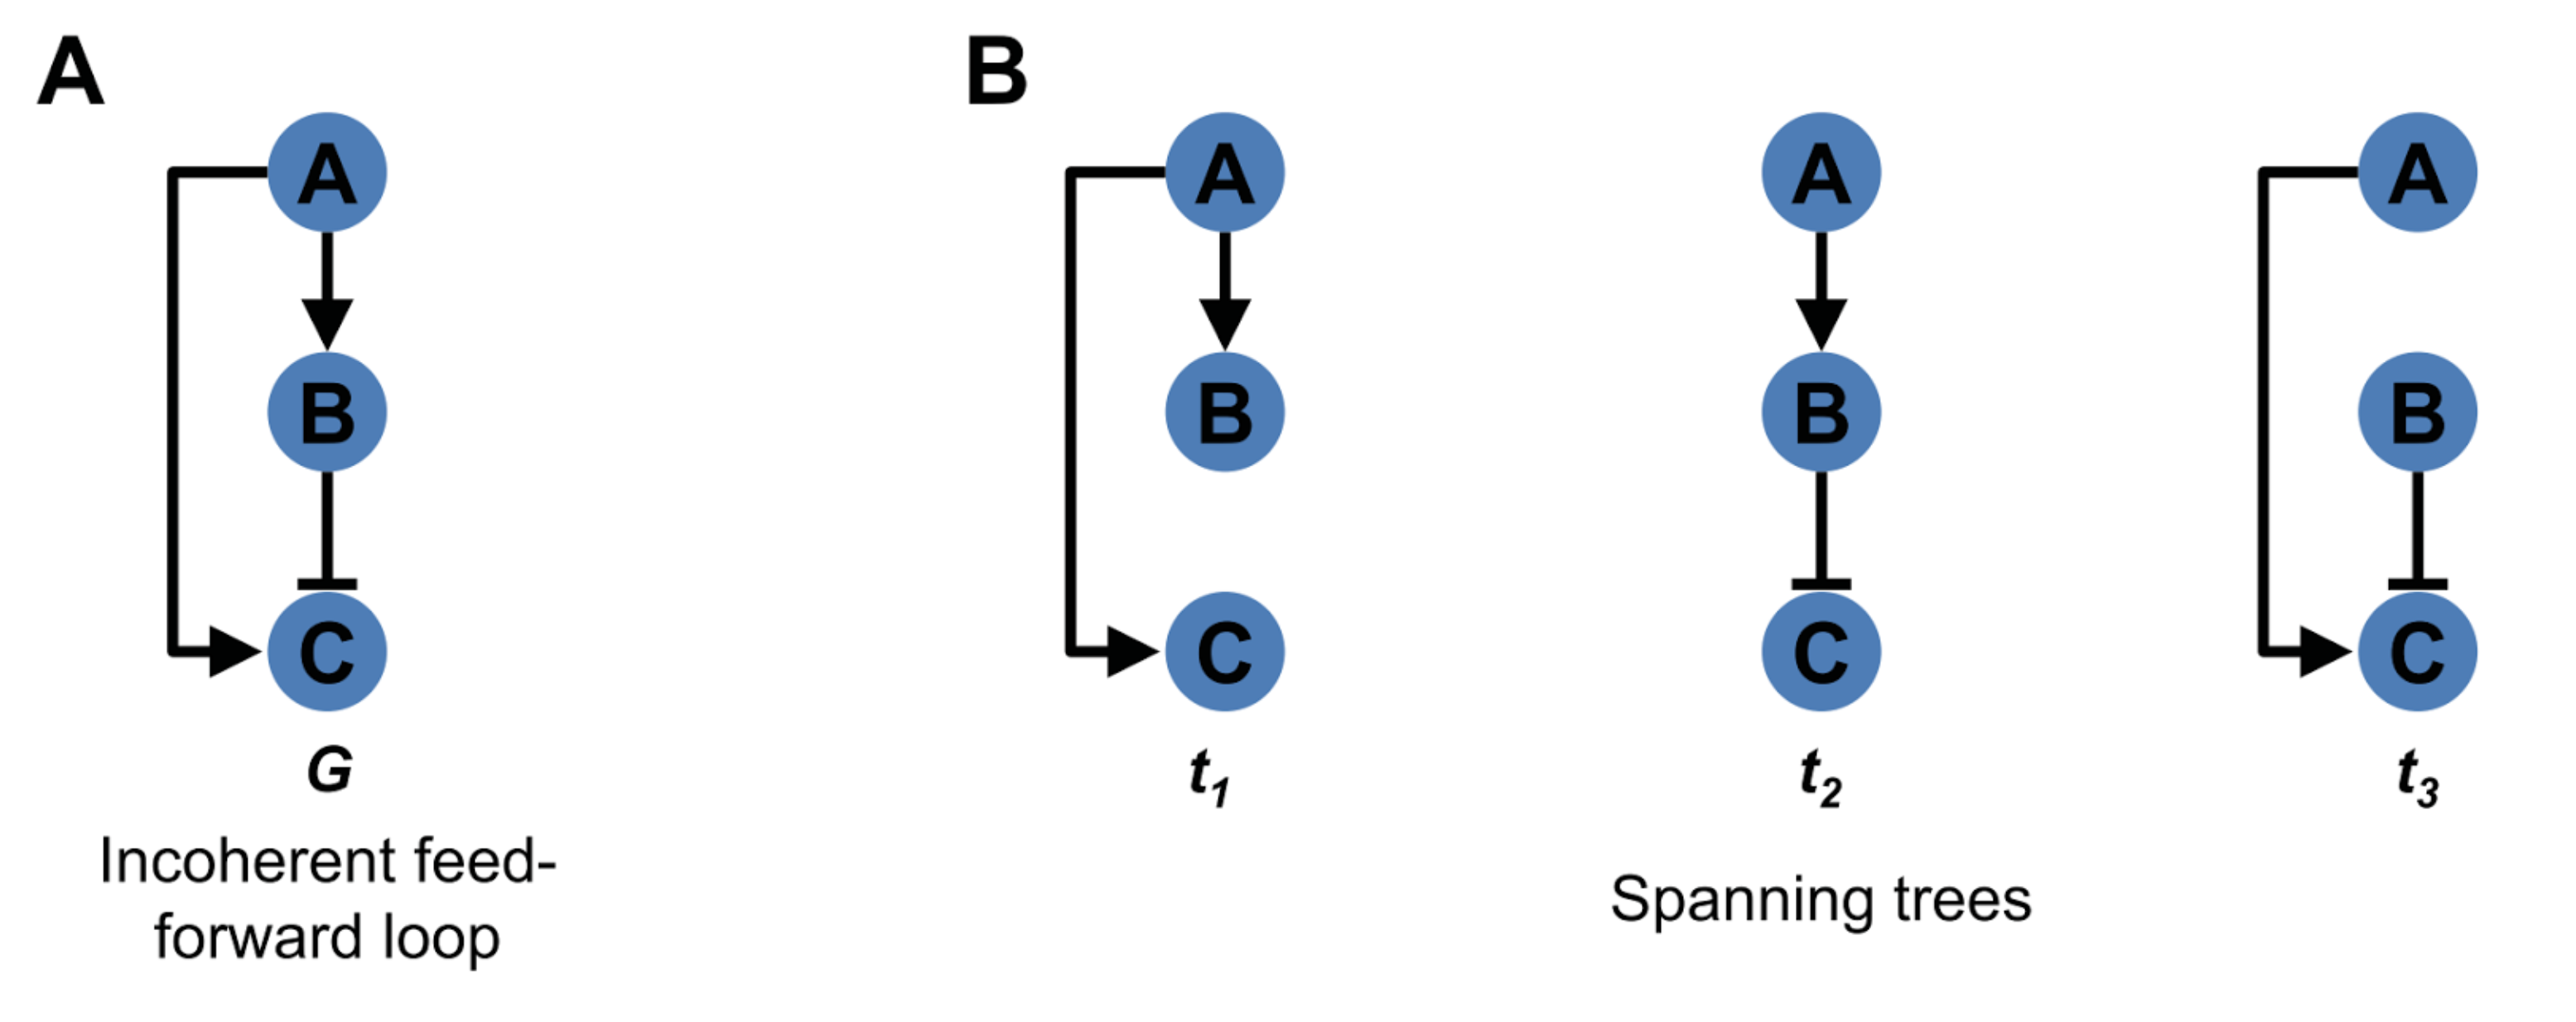
\includegraphics[width=160mm]{images/sst_example.png}}
\caption[Decomposition of Spanning Trees]{An example decomposition of a small causally inconsistent network A) to its spanning trees B)\cite{Vasilyev2014}.}
\label{Fig:sst_schematic}
\end{figure}

\subsection{Unsolved Issues}

While these algorithms already provide significant insight, they still have unresolved issues. For example: they require prior definitions of the upstream controller layer subnetworks; they do not address other exotic network motifs such as contradictions; and they do not take advantage of the vast assembly of correlative relationships. Further, there is generally a low coverage of nodes present in data sets within knowledge assemblies.

As mentioned before, these algorithms were developed for domains (oncology, immunology, etc.) that are rich in molecular data and mechanistic knowledge. For disease areas such as neurodegenerative diseases, molecular data (e.g., microarray, \ac{RNA}-seq) are not often available for the most applicable cells or tissues because of the practical difficulty of acquiring samples. It follows that context-specific knowledge is also much more sparse; and inference from other contexts (such as animal models) is much less reliable.

While backwards reasoning overcomes the issues with interpretation that are posed by forwards reasoning, the insufficient knowledge and data in neurodegenerative diseases makes this revelation much less useful. 

The experimental data available in for this field and other complex diseases are often multi-modal and multi-scale, prompting the development of new methods. Many of these experiments can only be connected to current knowledge assembles through correlative relationships, such as the associations between single nucleotide polymorphisms (\ac{SNP}s) and clinical phenotypes such as neuroimaging and gene expression. 

\section{A Priori Network Augmentation}

This section first describes pipelines that make biological knowledge assemblies more usable that rely on prior knowledge from the biomedical domain. Before developing analytical algorithms, it is first necessary to consider pipelines that improve the features of currently existing networks. After, an algorithm for generating upper layer controller networks is proposed and an alternative heat-diffusion method that is better able to accommodate heterogeneous experimental data. 

\subsection{Connecting Disconnected Components}

The GABA Subgraph in the Alzheimer's disease knowledge assembly has five disconnected components. While these can be inspected manually and the gaps can be filled, this becomes a daunting task for the set of 128 subgraphs in NeuroMMSig. PyBEL can be used to build queries that automatically expand and enrich graphs in order to create an environment in which disparate knowledge can be assembled to elucidate mechanistic understanding. Below, a procedure for filling in the holes in a subgraph is outlined. 

First, the central dogma is inferred. This ensures the existence of the corresponding RNA for proteins, and the corresponding genes for each \ac{RNA} and \ac{miRNA}. Doing so already connects the subgraph containing the relations describing how estradiol affects the expression of GABRA4 and GABR3 \ac{mRNA} \cite{Noriega2010} to another component that describes the functional impact of their translated proteins on other proteins and biological processes. After this process, four components remain.

Next, unqualified edges are enriched. This method reasons over nodes for which assertions can automatically be presumed. Relationships describing the different types of variations on genes and proteins (epigenetics, mutations, and post-translational modifications) are able to connect the GRIN2B node that is important in one large component to the phosphorylated GRIN2B node in another network. Because \ac{BEL} represents knowledge assemblies and not necessarily mechanistic models, these pieces of information can come from multiple curators without mutual knowledge. After this process, two components remain.

Of the two components, there is one large component and one small component, consisting only of cAMP catabolic process and GABBR2. While they are not yet automatic, further knowledge-based approaches can be used to connect GABBR2 to GABBR1 in the large component using resources like \ac{HGNC} Gene Families \cite{Gray2015}, InterPro \cite{Finn2017}, or PFAM \cite{Finn2016}. This is valuable because hierarchical knowledge sources like these can be used to reason over the network, like using the knowledge that GABBR2 decreases the cAMP catabolic process  \cite{Massone2011} to assert that GABBR1, the other member of the GPCR family 3, GABA-B receptor (IPR001828), shares the same activity. While this knowledge does not exist in the assembly, literature search also notes several connections between GABBR1 and cAMP signalling \cite{Frere2004,Palmer2005}.

\subsection{Subgraph Membership Inference}

While connecting components is important, it would also be useful to identify and add edges that should belong to the GABA subgraph but do not already. The first method would be to identify and edges occurring between nodes in the subgraph that are not already present, and add them. Next, this procedure can be continued to identify nodes that have edges to multiple nodes already in the subgraph. To reduce false positives, nodes added this way must both be the target of a causal relationship from a node in the subgraph and also have a causal effect on another node in the subgraph.

Finally, to improve viewability, two additional filters are provided. First, a filter for pathologies is used to remove them. This is useful since most pathologies are "super nodes" in knowledge assemblies and have numerous and often uninformative correlative relationships. Next, the central dogma is collapsed such that genes, \ac{RNA}s, and proteins are all shown as one node. While this limits the mechanistic explanatory power of a visualization, it removes a significant amount of visual clutter. 

\subsection{Pipeline Building}

It may be reasonable for viewing purpose to additionally collapse nodes representing modifications to their reference node as well. The submodule \\ 
\verb|pybel-tools.mutation| contains large library of functions that can be chained together either manually, or with a pipeline builder to promote reusability by allowing uses to save their workflows and reuse them. 

\section{Data Driven Analysis}

\subsection{Unbiased Candidate Mechanism Generation}

There are many terms used to describe portions of biological networks including pathways, mechanisms, subgraphs. They all comprise of individual interactions that accumulate to a more complex function. Often, an interaction may be part of multiple of these features. Knowledge bases like \ac{KEGG}, Reactome, and WikiPathways organize interactions into pathways; but they all suffer from bias in the literature and from the knowledge of their curators. This section presents an algorithm for generating unbiased candidate mechanisms from a given knowledge assembly. The method is then compared to the NeuroMMSig knowledge base to identify its ability to reproduce dogmatic subgraphs and identify areas of the underlying knowledge assemblies that have yet to be annotated.

In biomedical knowledge assembly across scales, biological processes represent entire subnetworks of causal interactions through both time and space. The \ac{NeuroMMSig} knowledge base captures associative, correlative,  and causal relationships between genes and gene products and biological processes directly in BEL. Because biological processes implicitly represent functional subnetworks, they are an appealing starting point for automatically unbiased generating candidate mechanisms to be used by other algorithms. 

The upstream controllers of biological processes provide direct insight to their functional impacts across scales. Therefore, the simple algorithm for generating candidate mechanisms that are unbiased by the dogmatic  takes the causally upstream controllers of a biological process, their upstream controllers, and all internal causal edges between them as a candidate mechanism. This method is thresholded at an expansion of two neighborhoods, but could easily be modified to choose larger or smaller lengths.

\subsection{Comparison to NeuroMMSig Knowledge Base}

This method was applied to the NeuroMMSig Alzheimer's disease knowledge assembly for each biological process. After, the resulting candidate mechanisms are compared to the NeuroMMSig subgraphs. First, the landscape of biological process membership in each subgraph is summarized with Figure 16. 

\begin{figure}
\captionsetup{format=plain}
\makebox[\textwidth]{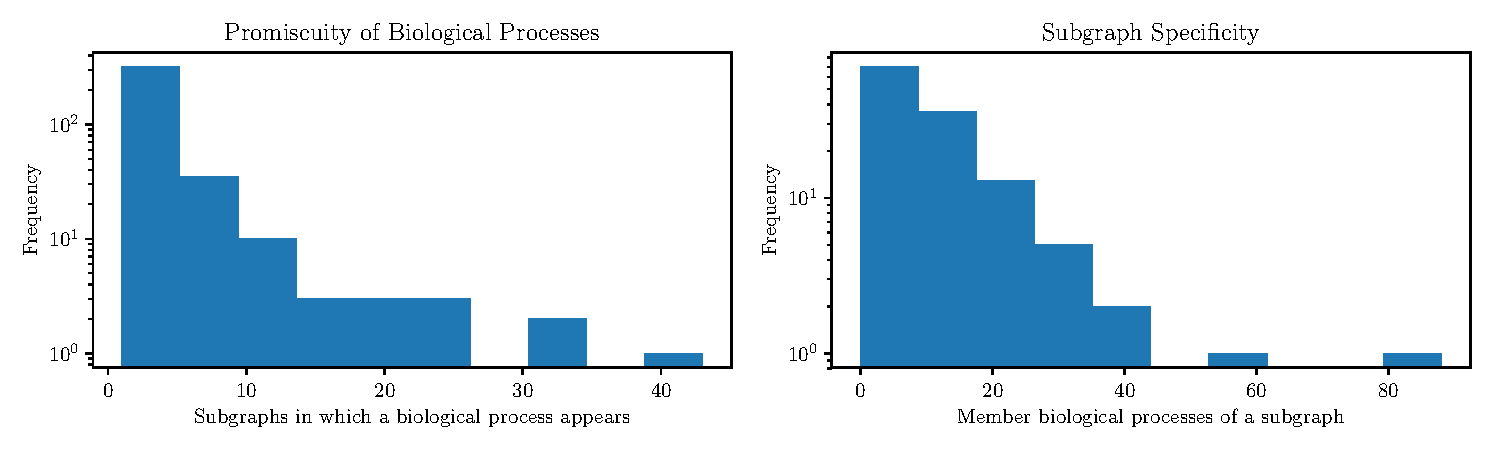
\includegraphics[width=160mm]{images/sg_comparison.pdf}}
\caption[The Landscape of Biological Process Membership in NeuroMMSig Subgraphs]{The landscape of biological process membership shows that there are both biological processes that appear in few and many subgraphs, and subgraphs with few and many biological processes.}
\label{Fig:sg_comparison}
\end{figure}

\begin{figure}
\captionsetup{format=plain}
\makebox[\textwidth]{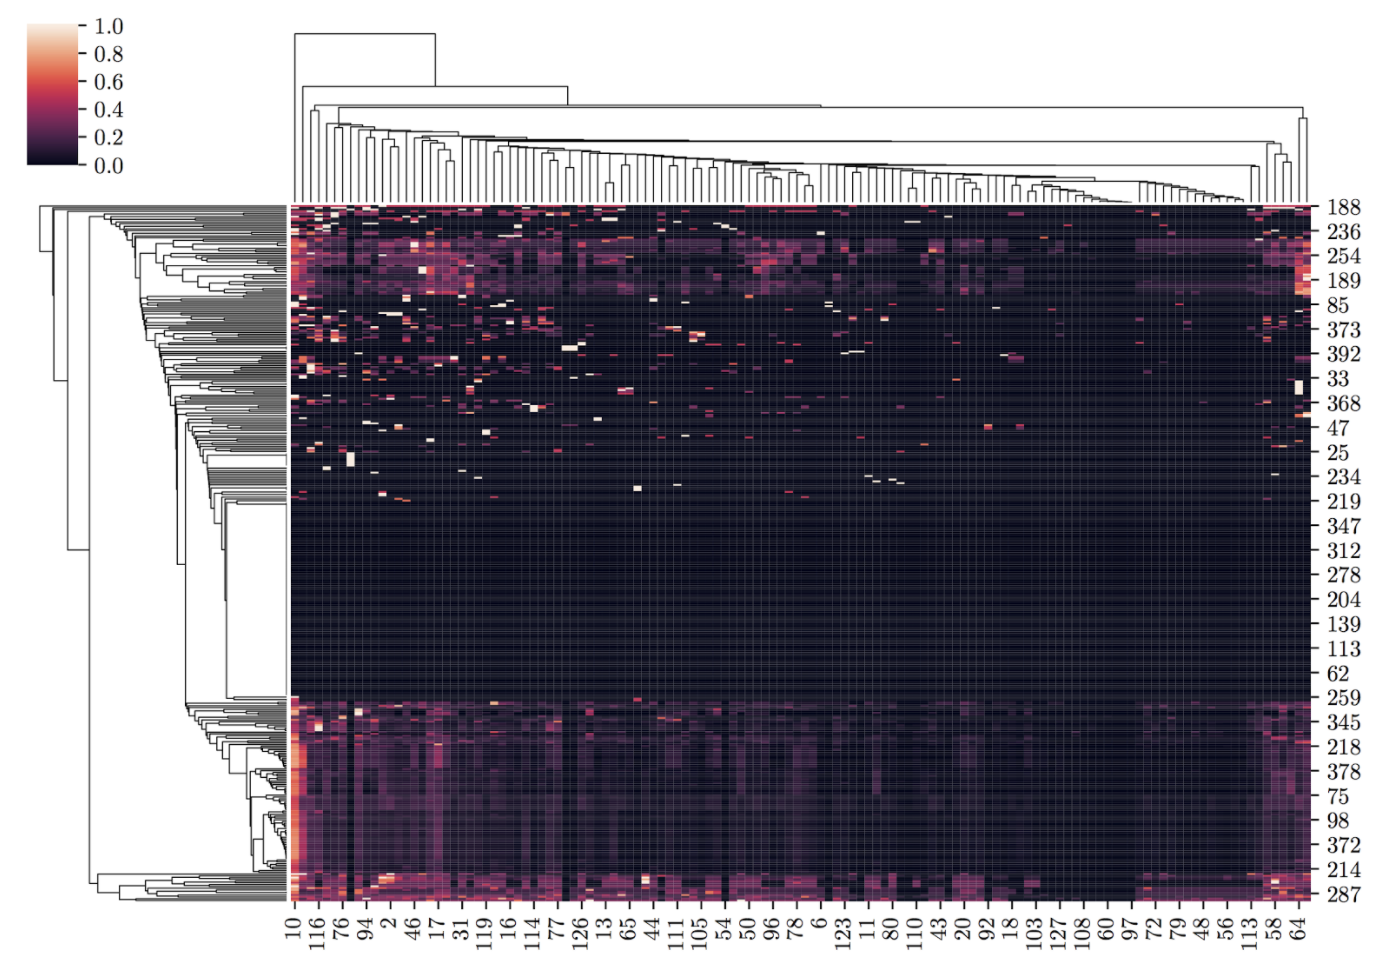
\includegraphics[width=160mm]{images/neurommsig_overlaps.png}}
\caption[Summary of the Overlap of Candidate Mechanisms with NeuroMMSig Subgraphs]{The landscape of candidate mechanism and \ac{NeuroMMSig} overlap, calculated by node overlap. The dark horizontal section directly identifies biological processes that are not annotated in any \ac{NeuroMMSig} subgraphs. This implicates their huge explanatory potential since they are outside the research dogma in Alzheimer's disease research.}
\label{Fig:neurommsig_overlaps}
\end{figure}

This landscape can also be used to annotate new candidate mechanisms to the dogmatic subgraphs in \ac{NeuroMMSig} to allow for more relevant mechanistic analysis. The annotation of further biological processes to subgraphs (Figure 17) can also allow the enrichment strategies in the \ac{NeuroMMSig} Mechanism Enrichment Server to perform enrichment over nodes corresponding to concepts on other scales.

\subsection{Candidate Mechanism Perturbation Amplitude}

All of the previous ideas from this thesis cumulate in the ability to devise and implement an algorithm for data-driven, schema-free analysis of networks. After networks are curated, parsed, enriched, checked for robustness, and triaged into unbiased candidate mechanisms, they can finally be analyzed. This section presents the candidate mechanism perturbation amplitude algorithm. It addresses the issues posed by previous algorithms with more complex randomized approaches and ultimately enables analysis of new modes of data by using a classical schema-free analytical technique similar inspired by other heat diffusion analyses in networks biology \cite{Bernabo2014,Leiserson2015}. The example presented below includes the use of differential gene expression analysis from Alzheimer's disease applied to the unbiased candidate mechanisms generated from the \ac{NeuroMMSig} knowledge assembly.

In this algorithm, heat is applied to the nodes based on the data set. For the differential gene expression experiment, the log-fold-change values were used instead of the corrected p-values to allow for the effects of up- and down-regulation to be admitted in the analysis. Finally, heat diffusion was run with the constraint that decreases edges cause the sign of the heat to be flipped. Because of the construction of unbiased candidate mechanisms, all heat will flow towards their seed biological process nodes. The amount of heat on the biological process node after heat diffusion stops becomes the score for the whole candidate mechanism.

Because heat always flows towards the biological process node, it is possible to remove leaf nodes (nodes with no incoming edges) after each step, since their heat will never change. 

The issue of inconsistent causal networks addressed by the SST algorithm does not affect heat diffusion algorithms since it can quantify multiple conflicting pathways. However, it does not address the possibility of contradictory edges, for example, when A increases B and A decreases B are both true. A random sampling approach is used on networks with contradictory edges and aggregate statistics over multiple trials are used to assess the robustness of the scores as a function of the topology of the underlying candidate mechanisms.

Finally, this algorithm can be tuned to allow the use of correlative relationships. Because many multi-scale and multi-modal data are often measured with correlations to molecular features, this enables experiments to be run using SNP or brain imaging features, whose experiments often measure their correlation with the activity of gene products. 

\subsection{Application Scenario}

This algorithm was applied with the Alzheimer's disease knowledge assembly to assist in interpretation of the differential gene expression experiments from GSE28146 \cite{Blalock2011}. This trial classified patients into three disease progression stages: early, moderate, and severe. While BEL has inherent limits in its temporal expressivity, interpreting data that has an inherent temporal ordering helps overcome this limit. The results for each time point can be accessed at \verb|https://github.com/pybel/pybel-notebooks/blob/master/results/time_series_cmpa.csv|.

\begin{figure}
\captionsetup{format=plain}
\makebox[\textwidth]{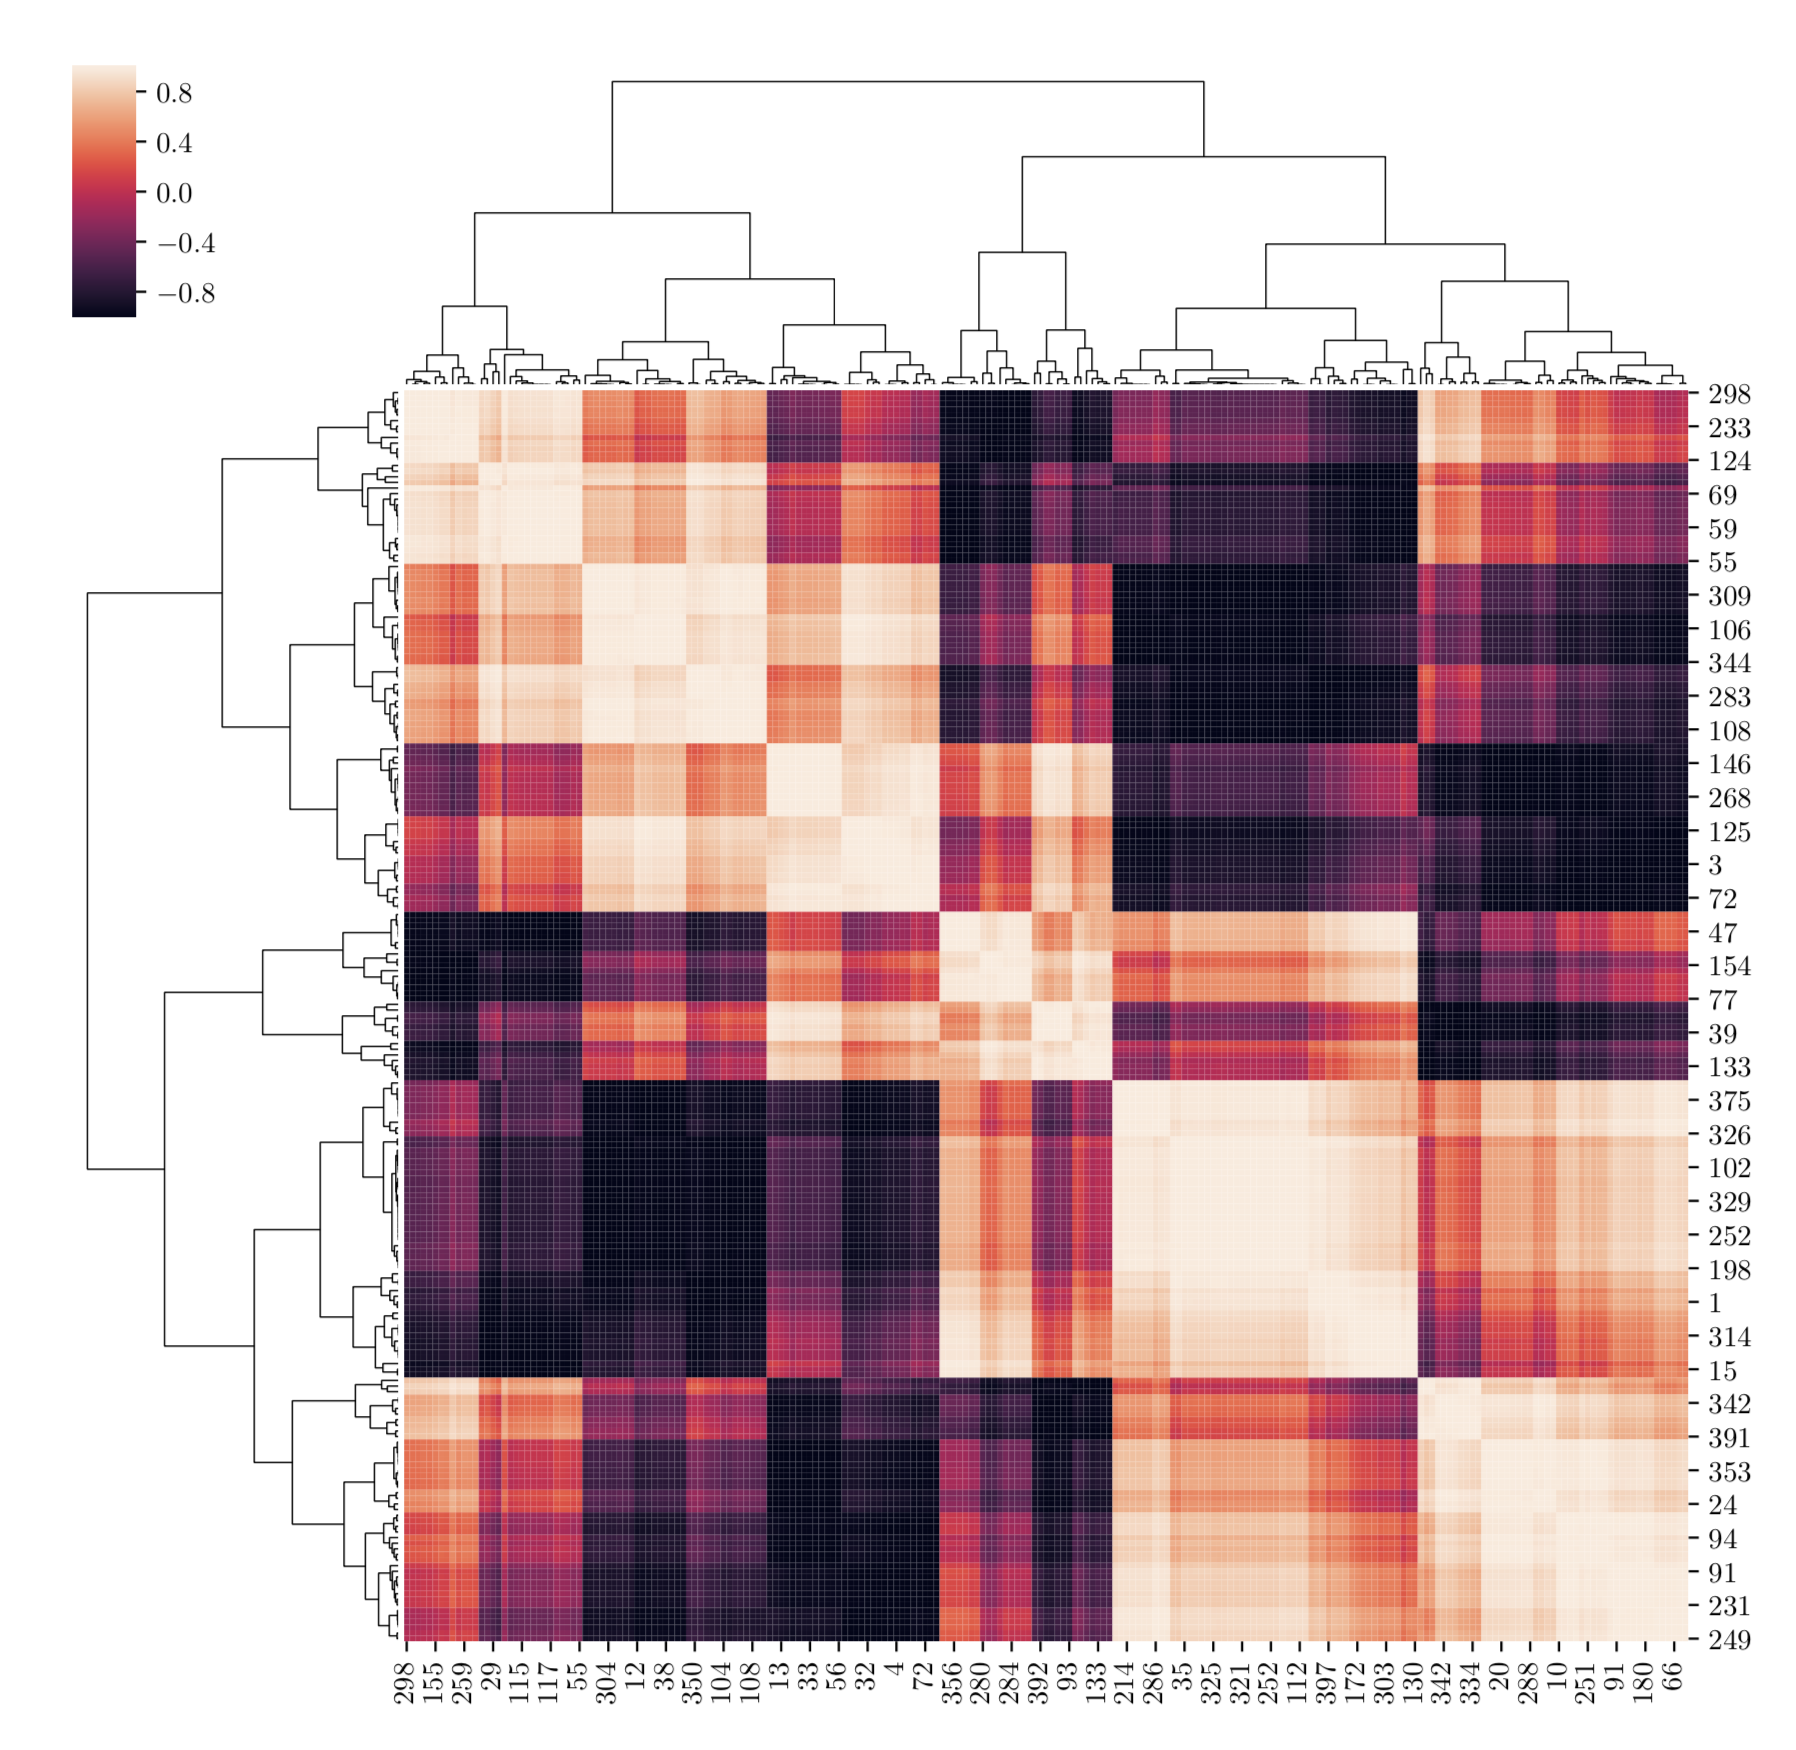
\includegraphics[width=160mm]{images/time_series_clustering.png}}
\caption[Clustering of Time-series Candidate Mechanism Perturbation Amplitude Scores]{A hierarchical clustering over the Pearson correlation of each candidate mechanism score through time suggests there are 4-6 discernible classes.}
\label{Fig:time_series_clustering}
\end{figure}

\begin{figure}
\captionsetup{format=plain}
\makebox[\textwidth]{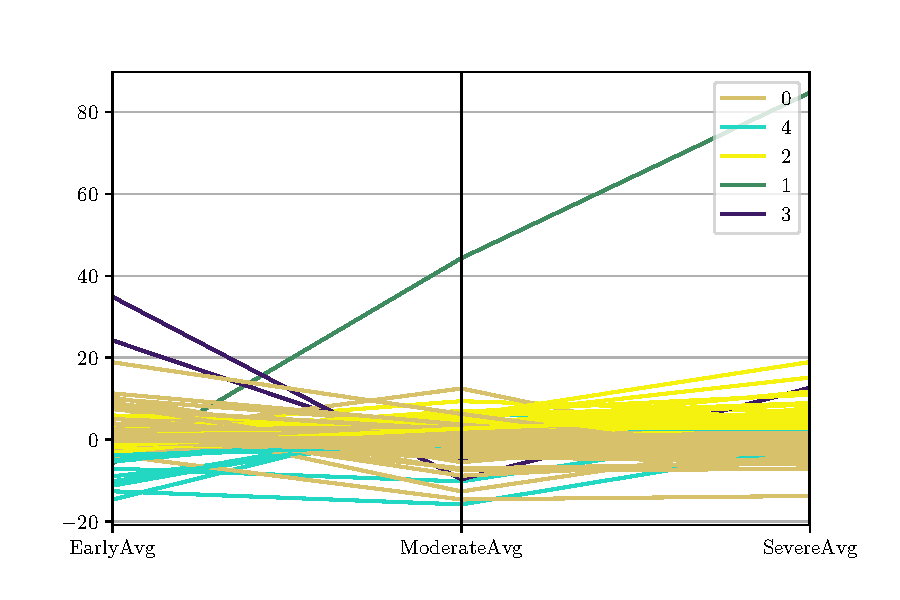
\includegraphics[width=120mm]{images/time_series_pc.pdf}}
\caption[Time-series Candidate Mechanism Perturbation Amplitude Score]{Parallel coordinate plot of all candidate mechanism with coloring by cluster shows the different progressions of biological processes.}
\label{Fig:time_series_pc}
\end{figure}

A hierarchical clustering (Figure 18) was performed using the Pearson correlation coefficient to group biological processes whose observed perturbation changed similarly through time. The dendrogram suggested there were between 4-6 groups of similarly varying processes. In order to make an interpretation, the original values are displayed in a parallel coordinate plot (Figure 19) with colors corresponding to their classes.

In figure 19, class 1 (green) is consists of biological processes that continually increase throughout the progression of the disease. Notably, it contains the inflammatory response. Class 3 (purple) contains biological processes that decrease from the early to moderate stage then increase again. This refers to cell death and neuron death processes. Class 4 includes processes that are initially down-regulated then become less regulated, including mitochondrion-related pathways. Class 2 (yellow) includes processes that do not become disregulated until the severe onset of disease, and have much more variety from glutamate secretion to ion homeostatic processes to metabolic processes. The remaining class does not show significant regulation in any of the disease stages. 

While Alzheimer's disease must be studied with respect to its progression over time, this analysis can provide insight directly to measurements performed on a single time series. Those results provide a ranking that prioritizes the most up- and down-regulated biological processes as a function of the observed data. 
